\documentclass{beamer}

\usepackage{graphicx} % for images
\usepackage{multicol} % for columns

\usepackage{listings} % for code blocks
\lstset{frameround=fttt,
	basicstyle=\ttfamily,
}

\usetheme{metropolis}

\setbeamertemplate{navigation symbols}{%
	\usebeamerfont{footline}%
	\usebeamercolor[fg]{footline}%
	\hspace{1em}%
}


\title{
\includegraphics[width=0.5\linewidth]{CoderDojo.png}\\ CoderDojo Carindale}
\subtitle{Morning Session}
\author{Thomas Meng}

\begin{document}

\maketitle

\section{What is TIC-80?}
\begin{frame}
	\frametitle{TIC-80}
	\begin{center}
		
\includegraphics{logo64.png}
	\end{center}
	\begin{quotation}
	\small{TIC-80 is a fantasy computer for making, playing and sharing tiny games.

	There are built-in tools for development: code, sprites, maps, sound editors and the command line, which is enough to create a mini retro game. At the exit you will get a cartridge file, which can be stored and played on the website. 

		Also, the game can be packed into a player that works on all popular platforms and distribute as you wish. To make a retro styled game the whole process of creation takes place under some technical limitations: 240x136 pixels display, 16 color palette, 256 8x8 color sprites, 4 channel sound and etc.}
	\end{quotation}
	\hfill -The TIC-80 website.
\end{frame}

\begin{frame}
	\frametitle{Ok... but why?}
	I think TIC-80 is a fun and structured way to learn text based programming as opposed to drag and drop (like Scratch).

	Like Scratch, we will be following a tutorial each week you should end up with a neat game at the end. You will be given more powerful tools to create your game with but you will also have more power to shoot yourself in the foot (so to speak).
	\begin{center}
		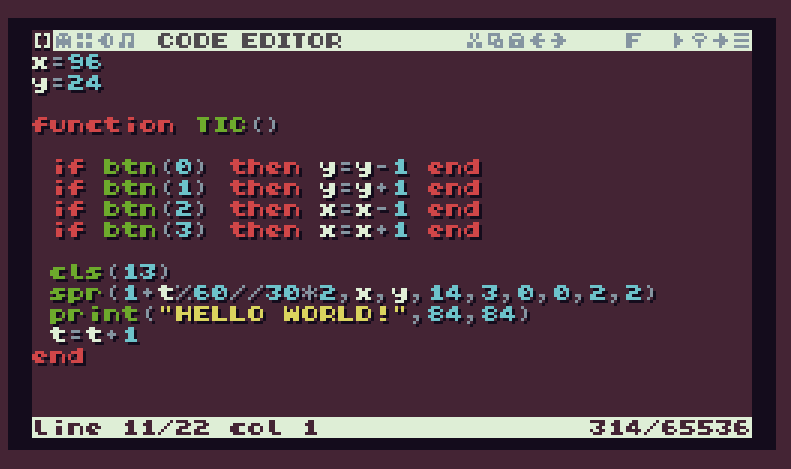
\includegraphics[width=0.5\linewidth]{enviro.png}
	\end{center}
\end{frame}

\begin{frame}
	\frametitle{Getting started}
	You are welcome to download the program if you have unstable internet or if it is running slowly.
	\begin{center}
		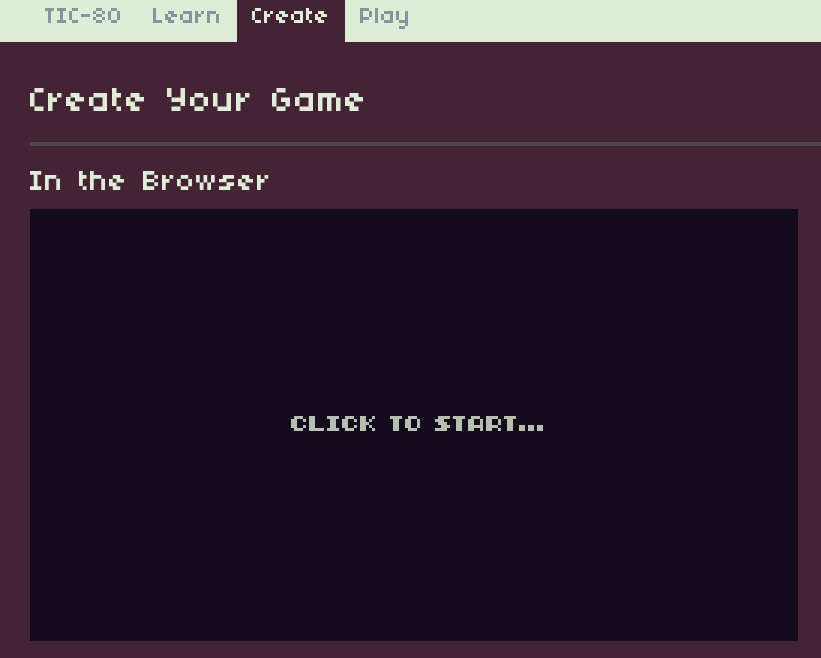
\includegraphics[width=0.7\linewidth]{starting.png}
	\end{center}
\end{frame}

\begin{frame}
	\frametitle{Creating your first TIC-80 game}
\end{frame}

\end{document}
